% Vorlage: https://www.pfsr.de/latex

% -- Anfang Präambel
\documentclass[german,  % Standardmäßig deutsche Eigenarten, englisch -> english
parskip=full,  % Absätze durch Leerzeile trennen
%bibliography=totoc,  % Literatur im Inhaltsverzeichnis (ist unüblich)
%draft,  % TODO: Entwurfsmodus -> entfernen für endgültige Version
]{scrartcl}

\usepackage[utf8]{inputenc}  % Kodierung der Datei
\usepackage[T1]{fontenc}  % Vollen Umfang der Schriftzeichen
\usepackage[main=english, ngerman]{babel} % Sprache auf Deutsch (neue Rechtschreibung)

% Mathematik und Größen
\usepackage{amsmath}
\usepackage[locale=DE,  % deutsche Eigenarten, englisch -> US
separate-uncertainty,  % Unsicherheiten seperat angeben (mit ±)
]{siunitx}
\usepackage{physics}  % Erstellung von Gleichungen vereinfachen

\usepackage{graphicx}  % Bilder einbinden \includegraphics{Pfad/zur/Datei(ohne Dateiendung)}

% Gestaltung
\usepackage{booktabs}  % schönere Tabellen
\usepackage[toc]{multitoc}  % mehrspaltiges Inhaltsverzeichnis
\usepackage{csquotes}  % Anführungszeichen mit \enquote
\usepackage{caption}  % Anpassung der Bildunterschriften, Tabellenüberschriften
\usepackage{subcaption}  % Unterabbildungen, Untertabellen, …
\usepackage{enumitem}  % Listen anpassen
\setlist{itemsep=-10pt}  % Abstände zwischen Listenpunkten verringern

% Manipulation des Seitenstils
\usepackage[headtopline = .5pt]{scrlayer-scrpage}

% Bibliographie
\usepackage[backend=biber]{biblatex}
\addbibresource{bibliography.bib}

% SI-Einheiten darstellen
\usepackage{siunitx}

% Kopf-/Fußzeilen setzen
\pagestyle{scrheadings}  % Stil für die Seite setzen
\clearmainofpairofpagestyles  % Stil zurücksetzen, um ihn neu zu definieren
\automark{section}  % Abschnittsnamen als Seitenbeschriftung verwenden
\ofoot{\pagemark}  % Seitenzahl außen in Fußzeile
\ihead{\headmark}  % Seitenbeschriftung mittig in Kopfzeile

\usepackage[hidelinks]{hyperref}  % Links und weitere PDF-Features

% TODO: Titel und Autor, … festlegen
\newcommand*{\titel}{Spectroscopy of Gamma Rays}
\newcommand*{\autor}{Sebastian Thiede, Alexander Lettau}
\newcommand*{\abk}{GA}
\newcommand*{\betreuer}{Yingjie Chu}
\newcommand*{\messung}{13.01.2022 \& 20.01.2022}
\newcommand*{\ort}{ASB/K07}

\hypersetup{pdfauthor={\autor}, pdftitle={\titel}}  % PDF-Metadaten setzen

% automatischen Titel konfigurieren
\titlehead{Praktikum des IKTP \abk \hfill TU Dresden}
\subject{Versuchsprotokoll}
\title{\titel}
\author{\autor}
\date{\begin{tabular}{ll}
Protokoll: & \today\\
Messung: & \messung\\
Ort: & \ort\\
Betreuer: & \betreuer\end{tabular}}

% -- Ende Präambel

\begin{document}
\begin{titlepage}
\maketitle  % Titel setzen
\tableofcontents  % Inhaltsverzeichnis setzen
\end{titlepage}

% ----- DOKUMENT ANFANG -----

\section{Calibration of a HPGE Detector}

\subsection{Calibration Curve}

In this part we were tasked with calibrating a HPGE-szintilator.
This calibration was done by a full energy peak analysis.
For this we took the gamma spectra of multiple sources, these were: $^{60}\text{Co}$, $^{137}\text{Cs}$, $^{133}\text{Ba}$ and $^{152}\text{Eu}$. 
In these spectra, we identified the photopeaks with the corresponding channels.
With the known energies and the identified channels, we could do a linear fitting, which gave us the linear energy-channel-relationship.

As a first measurement, the background radiation was measured for 15 days with the detector.
The result can be seen in Fig. \ref{hpge_background}
\begin{figure}[h]
  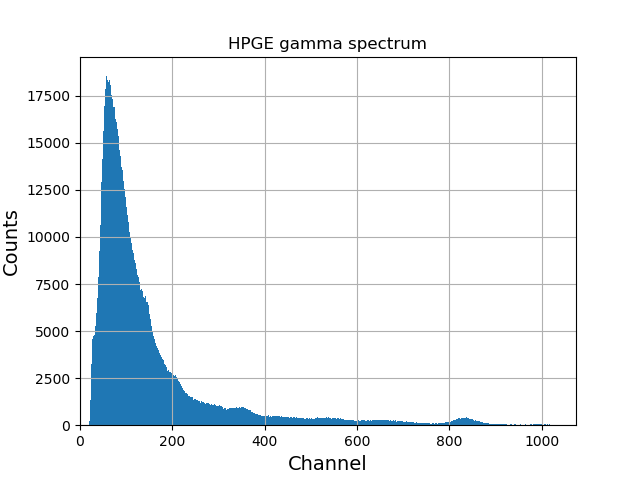
\includegraphics[width=\linewidth]{../Plots/hgpe_untergrund.png}
  \caption{Background radiation, measured for 15 days}
  \label{hpge_untergrund}
\end{figure}
For the analysis, we substracted the background sepctrum from the measured spectrum of the samples, to reduce the uncertainty.
Because the measured times for the samples were much lower, we rescaled the background for every sample with a factor $\frac{t}{15 \text{d}}$, with the measured time $t$. 
The resulting spectras can be seen in Fig. \ref{hpge}.
For the analysis, lets first analyse the spectrum of $^{137}$Cs and identify the specific structures.
In the outmost left and right, we can see peaks that result from decay radiation.
By comparision with (Quelle IAEA einfügen) we can identify the left peak, as resulting from beta-decay with a energy of $174$ keV and the left one from gamma-decay with a energy of $661$ keV.
In the middle, we can see two smaller peaks. These can again easily be identified as the compton edge to the right and the backscatter peak to the left with the compton contiuum in between.
For a full energy peak analysis, we are only interested in gammapeaks. 
The peak resulting from gamma-decay was marked and fitted by using a gaussian function:
\begin{equation}
N(K) = a \cdot exp \left( - \frac{(K - K_{0}^{2}}{2 \sigma ^{2}} \right)
\end {equation}
Where N are the counts and K is the channel.
From this fit, we used the mean value ($K_0$) as the channel, corresponding to the energy of the decay.
As a measurement of uncertainty, we used the $\textbf{full width at half maximum (FWHM)}$, which us defined as the width of a gaussian distribution at half height.
It can be calculated by:
\begin{equation}
\text{FWHM} = 2 \sqrt{2 \text{ln} 2} \sigma \approx 2.3548 \sigma
\end{equation}
This was done for every measured spectrum.
In every spectrum , we used one or two peaks with high intensity, which could be identified and distuinguished from other peaks.
The measurements and choosen peaks can be seen in Fig. \ref{hpge}.
The results of the fits can be seen in Fig. \ref{hpge_peaks}.

\begin{figure}[h]
\begin{subfigure}{.5\textwidth}
  \centering
  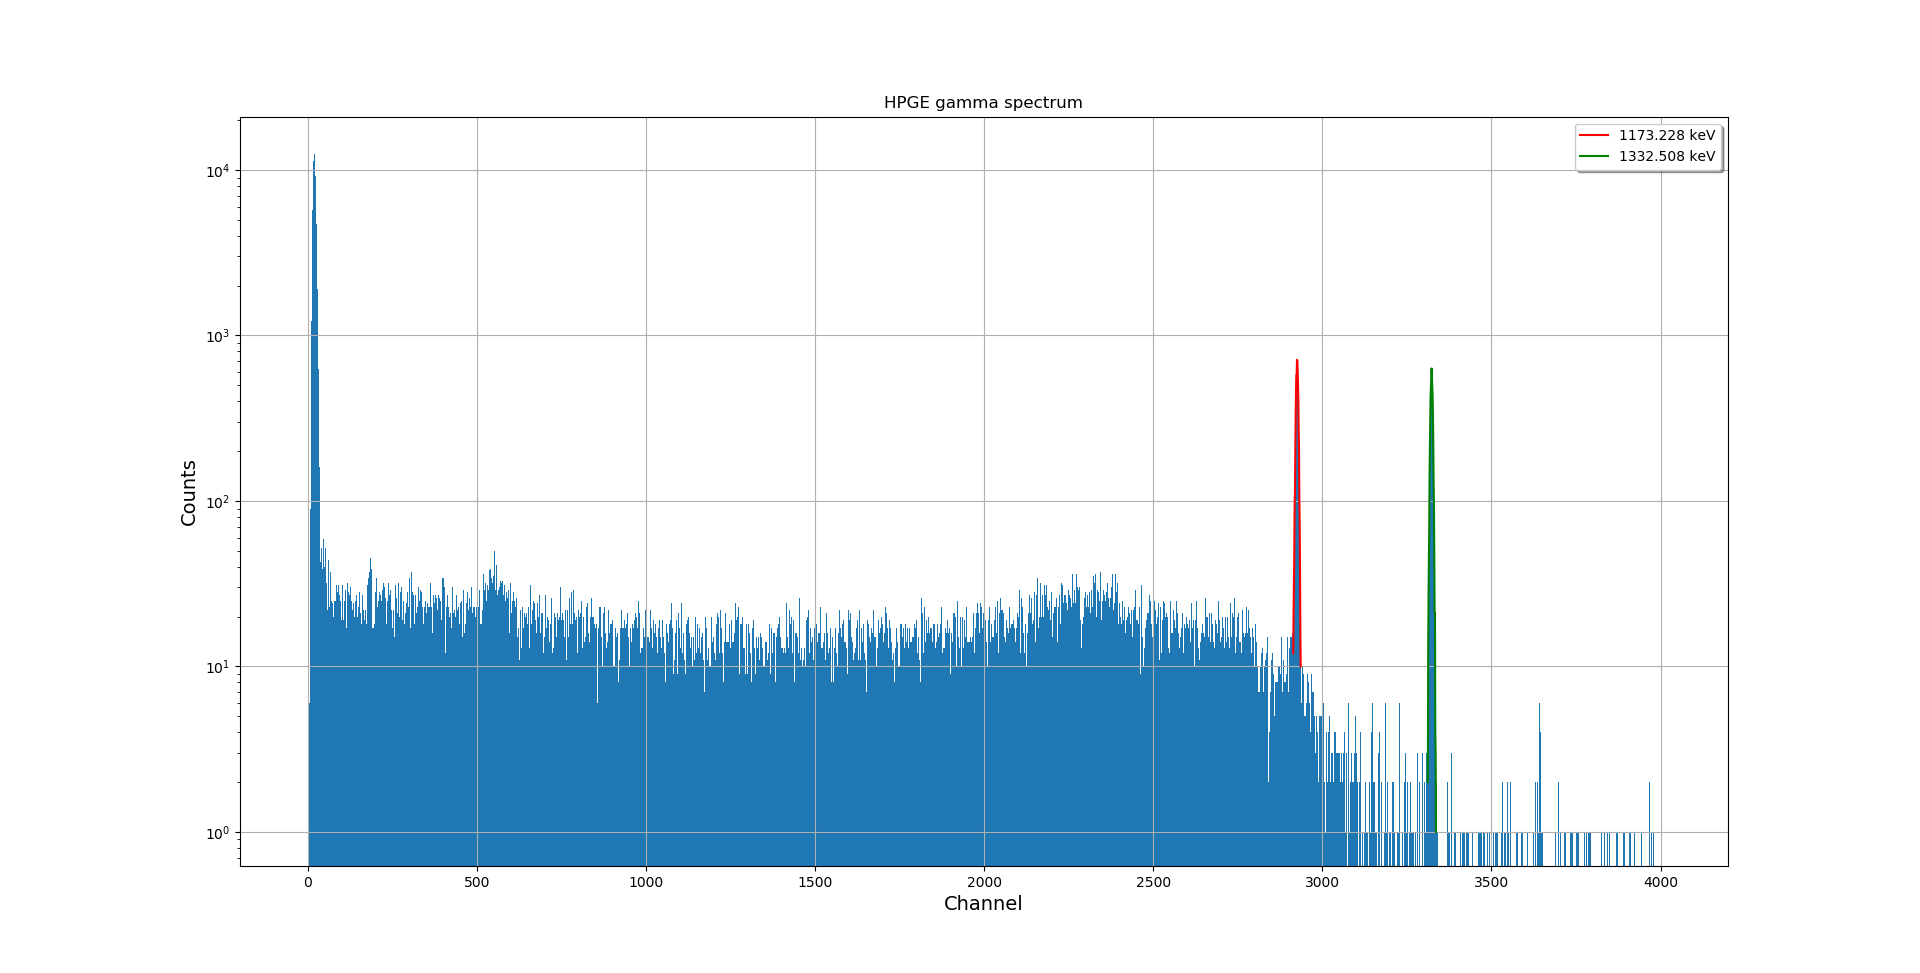
\includegraphics[width=.9\linewidth]{../Plots/hpge_co.png}
  \caption{$^{60}\text{Co}$}
\end{subfigure}%
\begin{subfigure}{.5\textwidth}
  \centering
  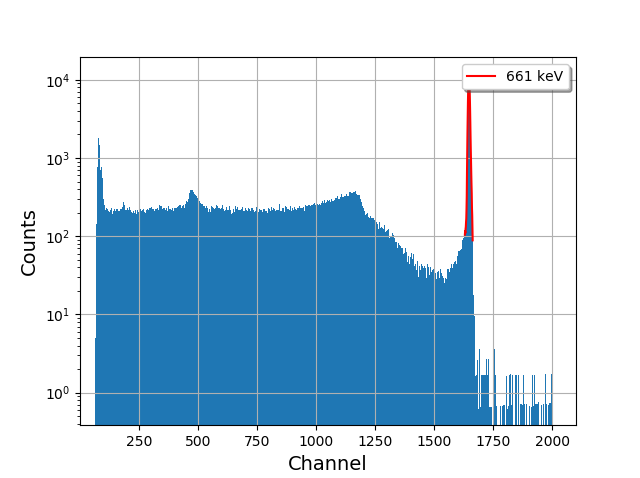
\includegraphics[width=.9\linewidth]{../Plots/hpge_cs.png}
  \caption{$^{137}\text{Cs}$}
\end{subfigure}%
 \vskip\baselineskip
\begin{subfigure}{.5\textwidth}
  \centering
  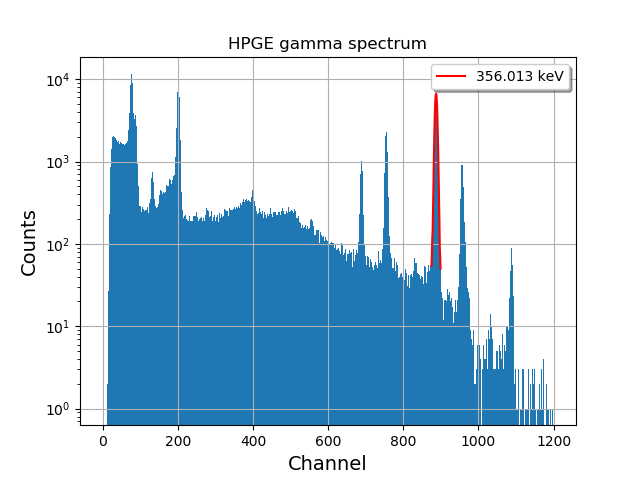
\includegraphics[width=.9\linewidth]{../Plots/hpge_ba.png}
  \caption{$^{133}\text{Ba}$}
\end{subfigure}%
\begin{subfigure}{.5\textwidth}
  \centering
  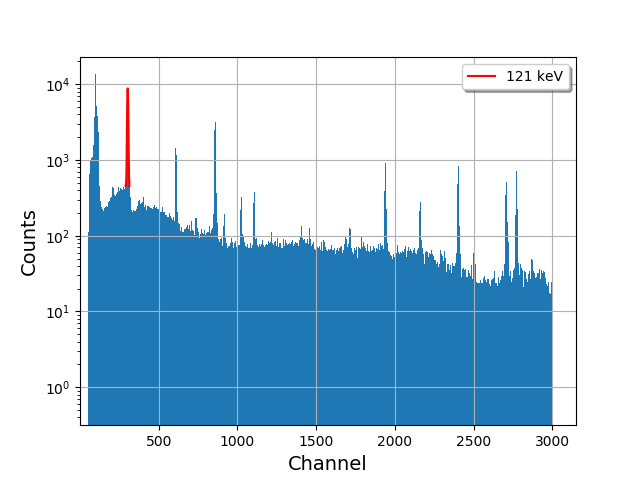
\includegraphics[width=.9\linewidth]{../Plots/hpge_eu.png}
  \caption{$^{152}\text{Eu}$}
\end{subfigure}%
\caption{gamma spectra of the measured sources}
\label{hpge}
\end{figure}

\begin{table}[h]
\centering
\begin{tabular}{c |c | c |c}
\hline
Isotop & $E_{\gamma}$ [keV]  & Channel & FWHM \\
\hline
$^{137}Cs$ & $661.657$ & 1647 & 8 \\
$^{60}Co$ & $1173.228$ & 2925 & 8 \\
$^{60}Co$ & $1332.508$  & 3323 & 8 \\
$^{152}Eu$ & $121.782$  & 303 & 7 \\
$^{133}Ba$ & $356.913$  & 887 & 7 \\
\hline
\end{tabular}
\caption{HPGE full energy peaks}
\label{hpge_peaks}
\end{table}

With the known energies and channels, we could now find the relationship between these for the HPGE detector.
For this we plotted the energy over the channels and made a linear fit. 
The parameters from the fitting gave us the relationship between these quantities.
The results can be seen in Fig. \ref{hpge_kali}

\begin{figure}[h]
  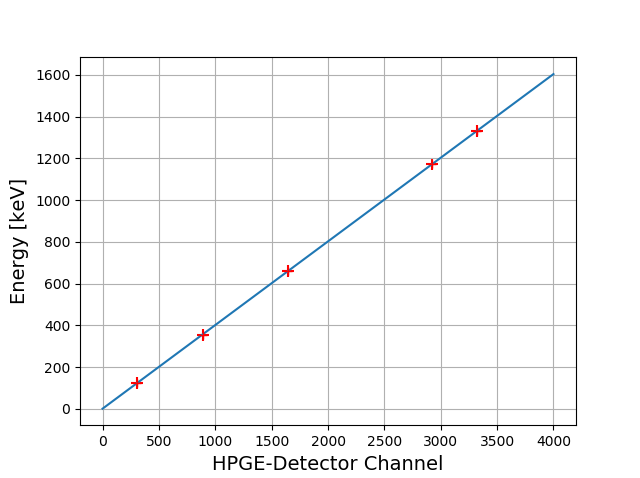
\includegraphics[width=\linewidth]{../Plots/hgpe_kali.png}
  \caption{Calibration curve of the HPGE detector}
  \label{hpge_kali}
\end{figure}
Fitparameters were calculated to a slope of $m = 0.40090 \pm 0.00020$ and an intercept of $n = 0.59 \pm 0,43$
Putting this all together gives us for the HPGE the calibration curve:
\begin{equation}
E(K) = [(0.40090 \pm 0.00020) \cdot K + (0.59 \pm 0.43)]  \text{keV}
\end {equation}

\clearpage

\subsection{Energy Resolution}

After we got the calibration curve, we looked into the energy resolution of the detector.
The energy resolution means how good peaks can be seperated from each other.
Peaks usually have a gaussian shape, so we can use the width of this curve as a measure of the resolution.
The energy resolution of a detector should follow the following formular:
\begin{equation}
\frac{\Delta E}{E} = \frac{\sqrt{a + bE + cE^2}}{E}
\label{resolution}
\end{equation}
In this formular, $\Delta E$ is the FHWM and $a$, $b$, $c$ are constants which describe different unvertainites from the detector.
From Eq. \ref{resolution} we get:
\begin{itemize}
\item $\frac{\Delta E}{E} \propto \frac{\sqrt{a}}{E}$ This term is caused by electronic noise inside the detector, background radiation or pile-up of multiple events.
\item $\frac{\Delta E}{E} \propto \frac{b}{\sqrt{E}}$  This terms follows statistical fluctuations during the detection.
\item $\frac{\Delta E}{E} \propto c$ This constant comes from inhomgeneities inside the detector, nonlinearrity of the detector or inter-calibration of detectors cells.
\end{itemize}
In the following part of the lab course, calculate these uncertainties  $a$, $b$, $c$.
The FHWM was already calculated for every peak in Tab. \ref{hpge_peaks}.
To get $\frac{\Delta E}{E}$ we have plotted the FHWM over the energy of the peaks.
These points were than fitted according to Eq. \ref{resolution}.
The result can be seen in Fig. \ref{hpge_res}.
Fitparameters were calculated to: $a = 47 \pm 5$, $b = -3.6 \pm 1.7$ and $c = 3.6 \pm 1.9$.

We can see, that Eq. \ref{resolution} is a good approximation for our data.
In the parameters we see, that the electronic noise seems to be the dominant uncertainty of the detector.
It is noticeable, that the calculated uncertainty for $b$ and $c$  are quite high.
This might be for numerical reasons, because of the fit function.


\begin{figure}[h]
  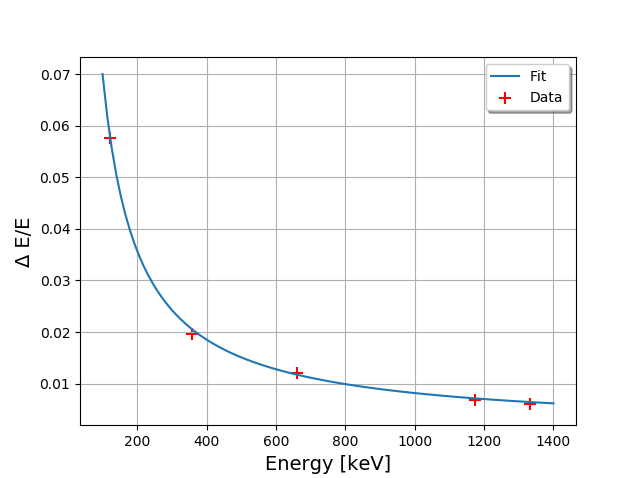
\includegraphics[width=\linewidth]{../Plots/hpge_resolution.png}
  \caption{Energy reslution of the HPGE detector}
  \label{hpge_res}
\end{figure}

\clearpage

\subsection{Peak Efficiency}
In the last part of the detector calibration, we will analiyse the peak efficiency of the detector.
The peak efficiency of a detector can be calculated for a detected peak as:
\begin{equation}
\eta = \frac{N_{obs}}{N_{emit}} = \frac{N_{obs}}{At_{live}P}
\end {equation}
With the observed counts for this peak $N_{obs}$, the acitivty of the sample $A$, the live time of the detector $t_{live}$ and the probability of this decay to happen $P$.
The observed counts can be calculated by integrating under the peak or, what we did, with the equation:
\begin{equation}
N_{obs} = I \sigma \sqrt{2\pi}
\label{gauss_area}
\end {equation}
Where $I$ is the amplitude of the peak and $\sigma$ is the standard deviation.
$A$ and $\sigma$ were calculated together with Tab. \ref{hpge_peaks}.
The probabilitys were taken from (iaea einfügen).

\begin{table}[h]
\centering
\begin{tabular}{c |c | c |c | c | c | c}
\hline
Isotop & $E_{\gamma}$ [keV] & $P$ & $t_{live}[s]$  & $A [kBq]$ & $N_{obs}$ & $\eta$ \\
\hline
$^{137}Cs$ & $661.657$ & 85.12  & 725   & $23.0 \pm 0.9$ & 96380  & $ (6.79 \pm 0.27)10^{-3}$ \\
$^{60}Co$ & $1173.228$ & 99.85  & 1206 & $1.09 \pm 0.04$ & 5872  & $ (4.47 \pm 0.18)10^{-3}$ \\
$^{60}Co$ & $1332.508$  & 99.98 & 1206 & $1.09 \pm 0.04$ & 5220  & $ (3.97 \pm 0.16)10^{-3}$ \\
$^{152}Eu$ & $121.782$  & 28.53 & 925   & $9.9 \pm 0.5$ & 62798    & $ (2.40 \pm 0.12)10^{-2}$\\
$^{133}Ba$ & $356.913$  & 62.05 & 971   & $7.3 \pm 0.4$ & 51132    & $ (1.163 \pm 0.037)10^{-2}$\\
\hline
\end{tabular}
\caption{HPGE full energy peaks}
\label{hpge_eff_calc}
\end{table}

This efficiency should in theory follow an exponential law:
\begin{equation}
\eta = a \cdot E^{-b}
\end {equation}
Ploting the calculated $\eta$ over the corresponding energies and fitting these points (see Fig. \ref{hgpe_eff} gave us the following peak efficiency of the HPGE detector:
\begin{figure}[h]
  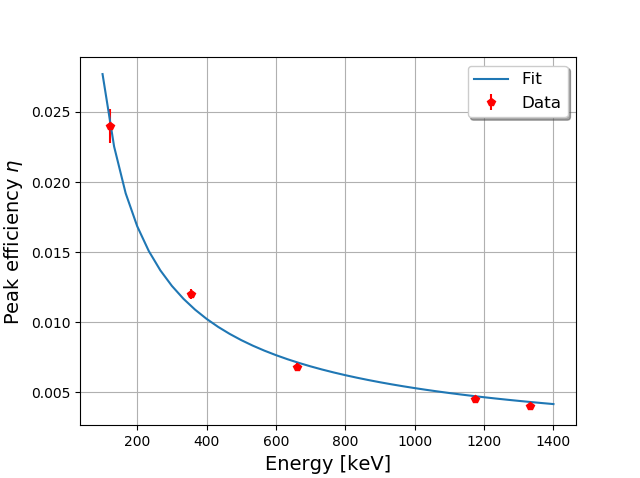
\includegraphics[width=\linewidth]{../Plots/hpge_eff.png}
  \caption{Peak efficiency of the HPGE detector}
  \label{hpge_eff}
\end{figure}
\begin{equation}
\eta = (0.755 \pm 0.014) \cdot E^{-(0.7174  \pm 0.0035)}
\label{peak_eff_eq}
\end {equation}

\clearpage

\section{Calibration of the NaI Scintilator}

Calibration of the NaI-scintilator was done analogous to the HPGE.
We used the same probes, exept for a new $^{22}$Na source, instead of $^{152}$Eu for another full energy peak analysis.
The probes were changed, because of the lower resolution fg the scintilator.

For this measurement we took a new measurement of the background radiation with the scintilator (see Fig. \ref{back_nai}.

\begin{figure}[h]
  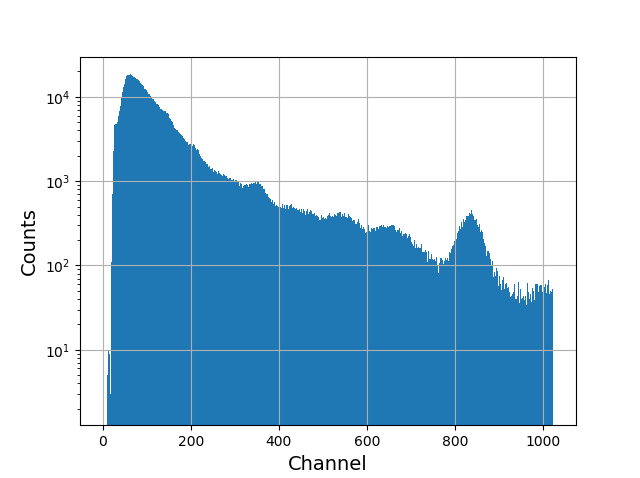
\includegraphics[width=\linewidth]{pictures/szin_background.png}
  \caption{Background radiation measured with the NaI scintilator}
  \label{nai_untergrund}
\end{figure}

This background was again substracted from every measured spectrum.
The measured spectra can be seen in Fig. \ref{szin}.
For this measurement, we put the source directly on top of the detector.
Just from looking at the spectra, we can already see that this scintilator has a much lower resolution.
The energy of the peaks were again taken from (iaea einfügen).
One special case here is with the $^{22}$Na sample.
In this spectrum we can't see any good gamma peaks.
The one we used, with an energy of $511$ keV has it's origin in photons that are created by annihilation of electrons und positrons, which are created by beta decay of $^{22}$N.

\begin{figure}[h]
\begin{subfigure}{.5\textwidth}
  \centering
  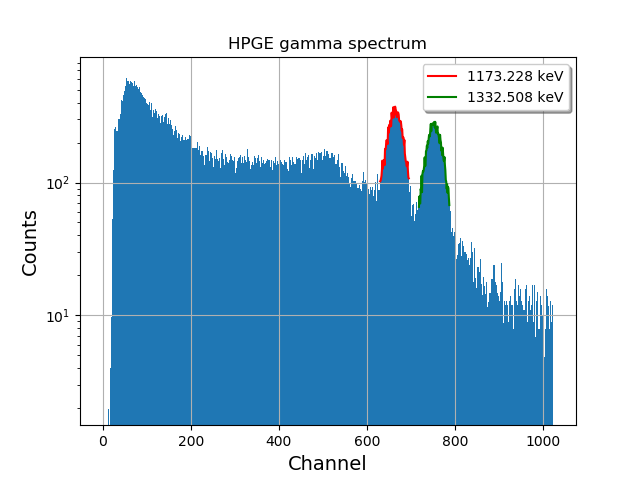
\includegraphics[width=.9\linewidth]{../plots/szin_co.png}
  \caption{$^{60}\text{Co}$}
\end{subfigure}%
\begin{subfigure}{.5\textwidth}
  \centering
  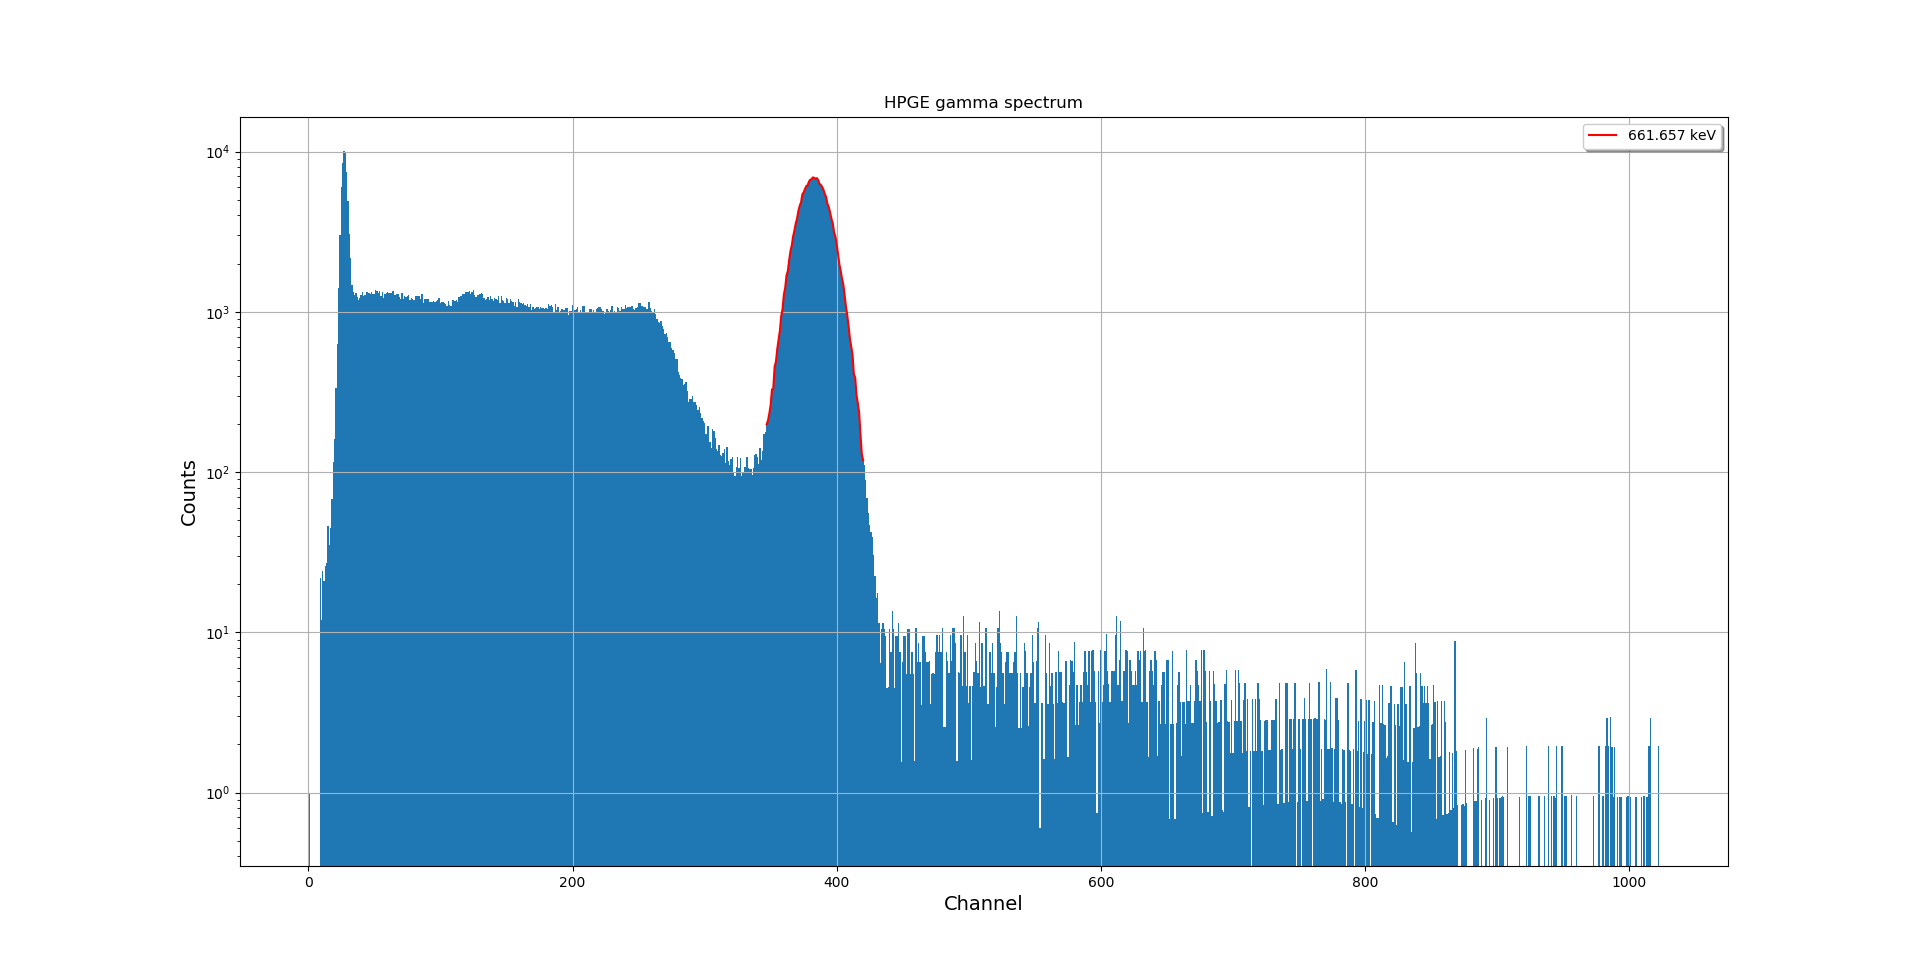
\includegraphics[width=.9\linewidth]{../plots/szin_cs.png}
  \caption{$^{137}\text{Cs}$}
\end{subfigure}%
 \vskip\baselineskip
\begin{subfigure}{.5\textwidth}
  \centering
  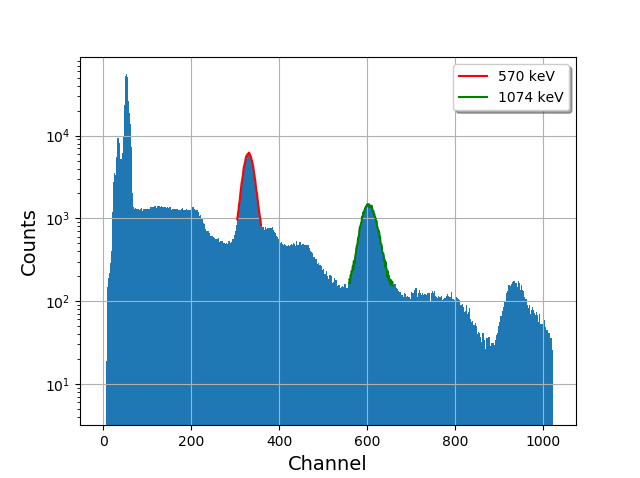
\includegraphics[width=.9\linewidth]{../plots/szin_bi.png}
  \caption{$^{207}\text{Ba}$}
\end{subfigure}%
\begin{subfigure}{.5\textwidth}
  \centering
  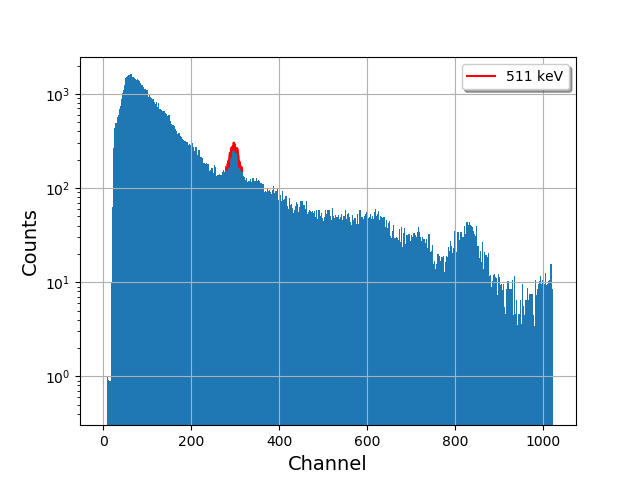
\includegraphics[width=.9\linewidth]{../plots/szin_na.png}
  \caption{$^{22}\text{Na}$}
\end{subfigure}%
\caption{gamma spectra of the measured sources}
\label{szin}
\end{figure}

We fitted the marked peaks again with a guassian function:
\begin{equation}
N(K) = a \cdot exp \left( - \frac{(K - K_{0}^{2}}{2 \sigma ^{2}} \right)
\end {equation}
Where $N$ are the counts and $K$ are the channels.
This gave us channels correspondig to a energy and the FHWM as measure of uncertainty.
The results can be seen in Tab, \ref{szin_peaks}.

\begin{table}[h]
\centering
\begin{tabular}{c |c | c |c}
\hline
Isotop & $E_{\gamma}$ [keV]  & Channel & FWHM \\
\hline
$^{137}Cs$ & $661.7$ & 383 & 29 \\
$^{60}Co$ & $1173.2$ & 664 & 27 \\
$^{60}Co$ & $1332.5$ & 753 & 39 \\
$^{207}Bi$ & $569.7$   & 331 & 27 \\
$^{207}Bi$ & $1063.7$ & 605 & 38 \\
$^{22}Na$ & $511.0$   & 298 & 23 \\
\hline
\end{tabular}
\caption{NaI full energy peaks}
\label{szin_peaks}
\end{table}
By plotting the enrgies over the channels we could again do a linear fit to find the relationship between these, for the NaI scintilator.
The results can be seen in Fig. \ref{szin_kali}

\begin{figure}[h]
  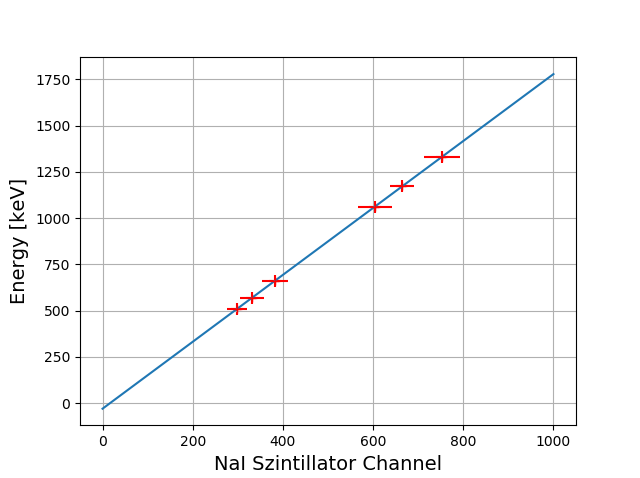
\includegraphics[width=\linewidth]{../plots/szin_kali.png}
  \caption{Calibration curve of the NaI scintilator}
  \label{szin_kali}
\end{figure}
Fitparameters were calculated to a slope of $m = 1.8084 \pm 0.0041$ and an intercept of $n = -29.6 \pm 2.2$
Putting this all together gives us for the scintilator the calibration curve:
\begin{equation}
E(K) = [(1.8084 \pm 0.0041) \cdot K - (29.6 \pm 2.2)]  \text{keV}
\end {equation}

\clearpage

\subsection{Energy Resolution}

With the calibration curve, we now looked into the energy resolution of the scintilator.
Just like for the HGPE detector, the resolution should be dependant on:
\begin{itemize}
\item an electronic noise term $a$
\item a term for statistical fluctioations $b$
\item a term for inhomgenieties in the detector $c$
\end{itemize}
For the NaI detector, the inhomogeneties should be of lesser concern for the uncertainty, which means that we will neglect $c$.
This modifies the theoretical function to:
\begin{equation}
\frac{\Delta E}{E} = \frac{\sqrt{a + bE }}{E}
\label{szin_resolution}
\end{equation}
As uncertainty for the energy ($\Delta E$) we used again the FHWM calculated in Tab. \ref{szin_peaks}.
Plotting $\frac{\Delta E}{E}$ und fitting according to Eq. \ref{szin_resolution} gave us Fig. \ref{szin_res}.

\begin{figure}[h]
  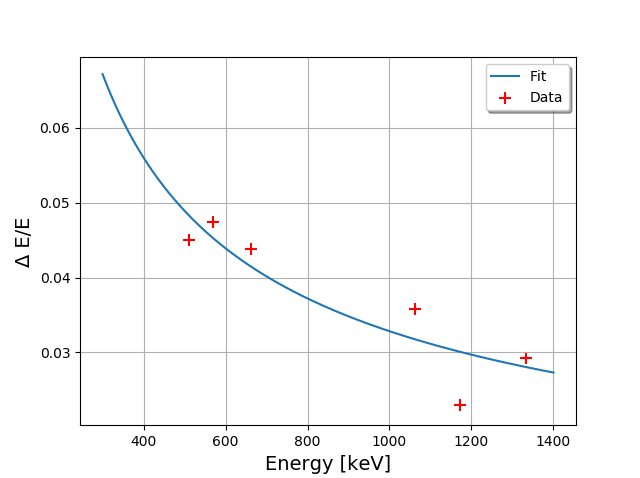
\includegraphics[width=\linewidth]{../plots/szin_res.png}
  \caption{Energy reslution of the NaI scintilator}
  \label{szin_res}
\end{figure}
With the fitting contsants: $a = 118 \pm 16$ and $b = 0.96 \pm 0.14$.
In Fig. \ref{szin_res} we can see, that the points have a pretty high deviation from the fit, yet in generell the function seems to work with the data.
This might have to do with the in generel high deviation of this scintilator.
Some more points for the fit should have made the result better.

\clearpage

 \section{Fukushima}

In the part, we were given a sample of leaves an gras from the region of Fukushima, which was contaminated with Caesium following the Fukushima nuclear disaster (11.03.2011).
The task was to calculate the date of the disaster, by using the activity ratio of $\frac{^{134}Cs}{^{137}Cs}$ from the sample.
In Fig. \ref{fukushima_spectrum} we can see the measured spectrum of the sample, where we again substracted background radiation.
\begin{figure}[h]
  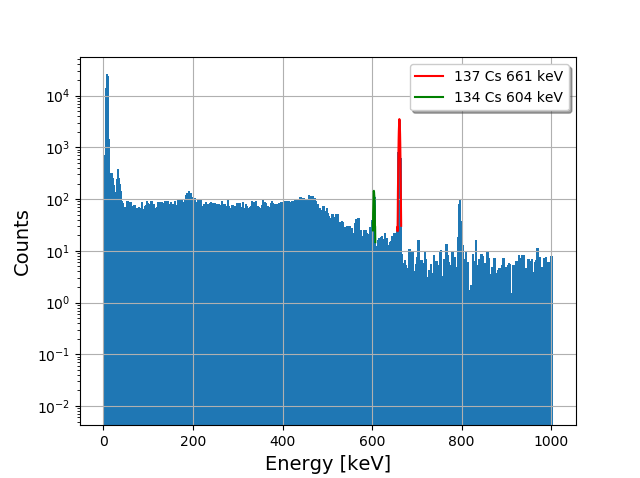
\includegraphics[width=\linewidth]{../Plots/fukushima_spektrum.png}
  \caption{Spectrum of the measured sample.}
  \label{fukushima_spectrum}
\end{figure}
Main interest in this spectrum lies in the peaks from $^{134}$ Cs, with $604$ keV and $^{137}$Cs with $661$ keV, which are marked in Fig. \ref{fukushima_spectrum}.
To calculate the age of the sample, we use the ratio of the activity of $\frac{^{134}Cs}{^{137}Cs}$:
\[
\frac{A_{134}}{A_{137}} = \frac{A_{134}^0}{A_{137}^0} \cdot \frac{e^{-t(\lambda_{134})}}{e^{-t(\lambda_{137})}}
\]
\[
= \frac{A_{134}^0}{A_{137}^0} \cdot e^{-t (\lambda_{134} - \lambda_{137})}
\]
\begin{equation}
\rightarrow t = \frac{ \text{ln} \left(\frac{A_{134} A_{137}^0}{A_{137} A_{134}^0}\right)}{\lambda_{134} - \lambda_{137}}
\label{time}
\end{equation}
With the acitivities of the isotopes during the measurement $A_i$, the acitivities during the accident $A_{i}^0$ and the decay rates $\lambda _i$.
The acivity at any point can be calculated as:
\begin{equation}
A_i (t) = \lambda \cdot N_i (t)
\end{equation}
With the number of particles $N_i$.
Putting this into Eq. \ref{time} gives us:
\begin{equation}
\rightarrow t = \frac{ \text{ln} \left(\frac{A_{134} N_{137}^0 \lambda_{134}}{A_{137} N_{134}^0 \lambda_{137}}\right)}{\lambda_{134} - \lambda_{137}}
\end{equation}
Which means, that we only need to know the abundance ratio of the isotopes.
This can be calculated with the production of these through fission and was given to us as: 
\[
 \frac{^{134}Cs}{^{137}Cs} = \frac{6 \%}{68\%}
\]
The activity of the sample was calculated with:
\begin{equation}
A_i = \frac{N_{obs}}{t_{live} \eta (E_i) P}
\end{equation}
With the area under the Peak $N_{obs}$, calculated with Eq. \ref{gauss_area}, the live time of the detector ($t_{live}=39508 \text{s}$), the peak efficiency for this energy ($\eta$), calculated with Eq. \ref{peak_eff_eq}  and the probabilities of the decays.
For the values in the calculation, we got:
\begin{table}[h]
\centering
\begin{tabular}{c |c | c |c }
\hline
$\text{Isotop}$ & $ \eta $ & $ A[\text{Bq}] $  & $ \lambda $ \\
\hline
$^{137}Cs$ & $(6.79 \pm 0.27) \cdot 10^{-3}$ & $46.353 \pm 0.098$ & $7.302 \cdot 10^{-10}$ \\
$^{134}Cs$ & $(7.64 \pm 0.14) \cdot 10^{-2}$ & $1,29 \pm 0.25$ & $1.064 \cdot 10^{-8}$ \\
\end{tabular}
\caption{Values for the calculation of $t$}
\end{table}
The probabilities were taken from(iaea einfügen) as: $P(604 \text{keV}) = 97 \%$ and $P(661 \text{keV}) = 85 \%$.

Putting this all together gives us:
$t = 11.83 \pm 0.20 \text{a}$
With the day of measurement (14.01.22), this would date the fukushima accident to the 14.03.2010.



\section{Unknown Samples}
In this part we got 5 samples of ashe from leaves and pines, from eastern europe.
Of these samples, we took the gamma spectrum with the HPGE detector and compared them with a refference sample.
The sample contains radioactive $^{137}$Cs which is supossed to be contained in the ashe, because of the Chernobyl nuclear accident.
In the following we compare the acitivty of $^{137}$Cs from the ashe with the refference.
From all spectra we substracted the background radiation.

In Fig. \ref{cher_samples} we can see the spectrum of the refference and the samples.
\begin{figure}[h]
\begin{subfigure}{.5\textwidth}
  \centering
  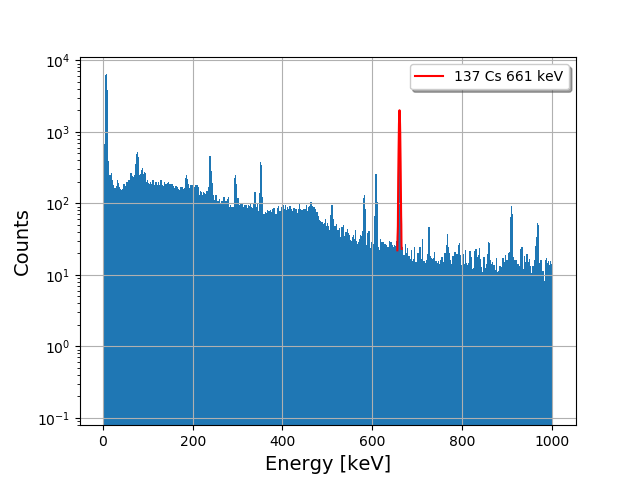
\includegraphics[width=.9\linewidth]{pictures/cher_ref.png}
  \caption{Reference sample}
\end{subfigure}%
\begin{subfigure}{.5\textwidth}
  \centering
  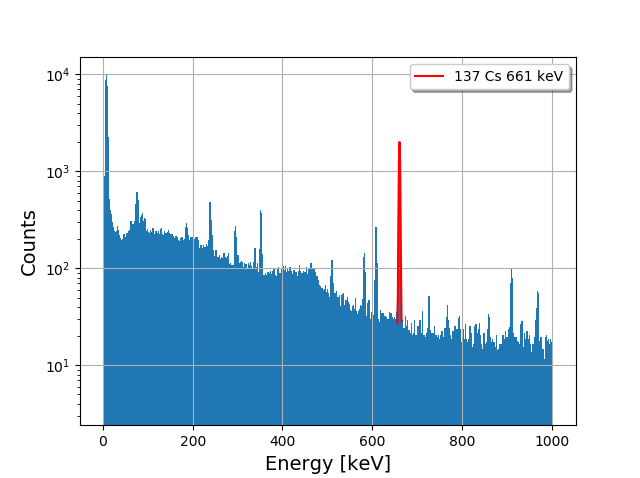
\includegraphics[width=.9\linewidth]{../plots/PP34R1_1.png}
  \caption{Sample $PP34R1\_1$}
\end{subfigure}%
 \vskip\baselineskip
\begin{subfigure}{.5\textwidth}
  \centering
  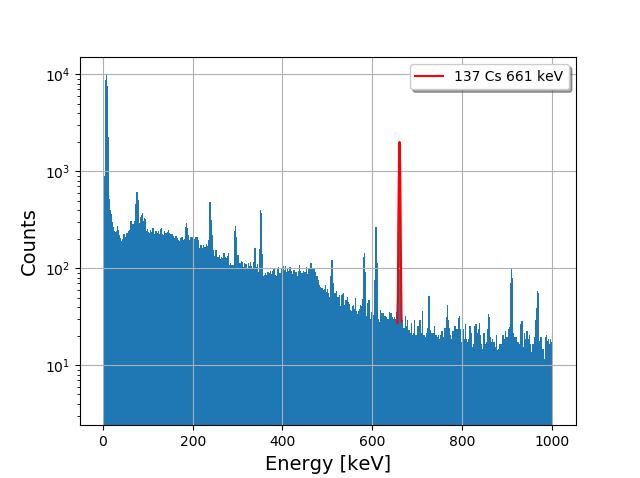
\includegraphics[width=.9\linewidth]{../plots/PP5PR1_2.png}
  \caption{Sample $PP5PR1\_2$}
\end{subfigure}%
\begin{subfigure}{.5\textwidth}
  \centering
  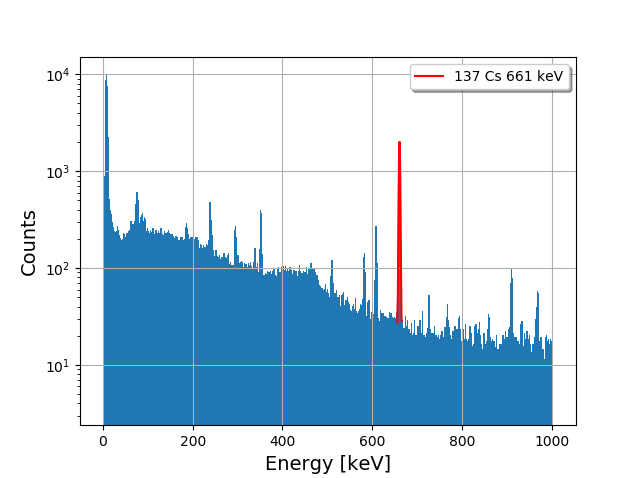
\includegraphics[width=.9\linewidth]{../plots/PP63R1_3.png}
  \caption{Sample $PP63R1\_3$}
\end{subfigure}%
 \vskip\baselineskip
\begin{subfigure}{.5\textwidth}
  \centering
  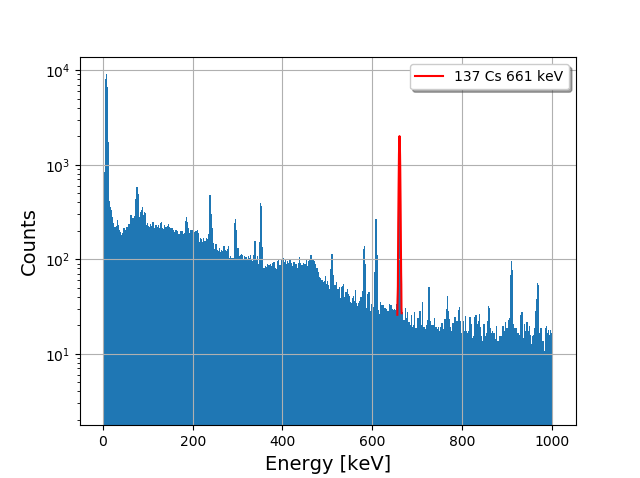
\includegraphics[width=.9\linewidth]{../plots/PP84R2_4.png}
  \caption{Sample $PP84R2\_4$}
\end{subfigure}%
\begin{subfigure}{.5\textwidth}
  \centering
  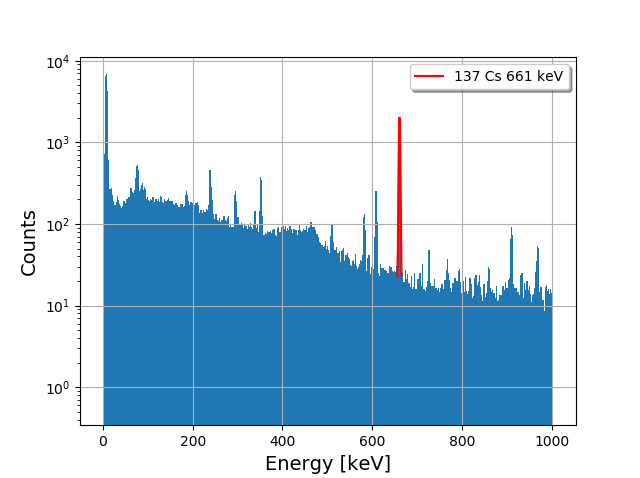
\includegraphics[width=.9\linewidth]{../plots/PPACR2_5.png}
  \caption{Sample $PPACR2\_5$}
\end{subfigure}%
\caption{gamma spectra of the measured samples}
\label{cher_samples}
\end{figure}
Measurement time was around 3h.
In every samples we can clearly  see a  $^{137}$Cs peak, together with smaller peaks.
Some of these smaller peaks might come from natural occuring isotopes, while some might result from the Chernobyl accident too.
For this analysis we will concentrate on $^{137}$Cs.

From the peaks we calculated the measured acitivty again as:
\begin{equation}
A_i = \frac{N_{obs}}{t_{live} \eta (E_i) P}
\end{equation}
The observed counts $N_{obs}$ were this time calculated as:
\begin{equation}
N_{obs} = \frac{I \sigma \sqrt{2 \cdot \pi}}{b}
\end{equation}
With the binwidth $b = 0.4$ to compensate the change of binwidth on the energy scale.
For the analysis we than took the ration $\frac{A_i}{A_0}$ with the activity of the reference $A_0$ and the activity of the samples $A_i$.
The results can be seen in Tab. \ref{cher_results}.
The uncertainties were calculated from the uncertainty of $N_{obs}$ and $\eta$.

\begin{table}[h]
\centering
\begin{tabular}{c |c | c }
\hline
Sample & A [Bq] & $\frac{A}{A_0}$ \\
\hline
Reference & $8.1 \pm 1.2   $ & $1$ \\
$PP34R1\_1  $& $113.7 \pm 1.3$ & $14.1 \pm 4.3$ \\
$PP5PR1\_2  $& $114.4 \pm 1.3$ & $14.2 \pm 4.4$ \\
$PP63R1\_3  $& $106.6 \pm 1.3$ & $13.2 \pm 4.0$ \\
$PP84R2\_4  $& $36.2 \pm 1.3  $ & $4.5 \pm 1.4$ \\
$PPACR2\_5 $& $14.4 \pm 1.3  $ & $1.8 \pm 1.4$ \\
\hline
\end{tabular}
\label{cher_results}
\end{table}
Every measured sample has a higher activity than the reference sample.
The lowest acitivity is with sample $PPACR2\_5$, which has nearly double the acitivity of the reference source.
Three of the samples ($PP34R1\_1, PP5PR1\_2 \text{and} PP63R1\_3$) have an activity more than ten times higher, which could mean, that these contain a considerable amount of radioactive  $^{137}$Cs.

\section{Attenuation}

In this part of the lab course, we investigated the attenuation of radiation from $^{137}$Cs through copper.
The attenuation of radiation can be calculated with:
\begin{equation}
I(d) = I_0 e^{\frac{\mu}{\rho} d  }
\end {equation}
Where $I$ is the attenuated quantity, $I_0$ is this quantity without attenuatiuon, $\frac{\mu}{\rho}$ is the mass attenuation coeficient and $d$ is the lenght over which the attenuation takes place.
To measure these, we took the spectra of $^{137}$Cs, shielded through multiple layers of copper.
Natural occuring copper only has stable isotopes, which means that this shielding shouldn't give much extra background radiation
The measured spectra can be seen in Fig. \ref{attenuation_spectra}.
\begin{figure}[h]
\begin{subfigure}{.5\textwidth}
  \centering
  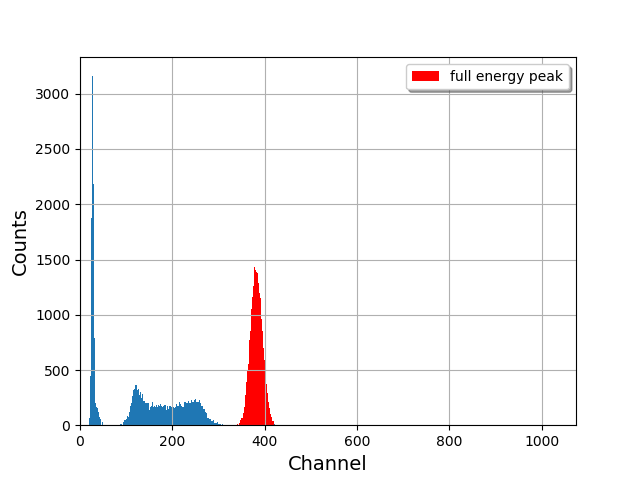
\includegraphics[width=.9\linewidth]{../Plots/attenuation_0.png}
  \caption{no copper}
\end{subfigure}%
\begin{subfigure}{.5\textwidth}
  \centering
  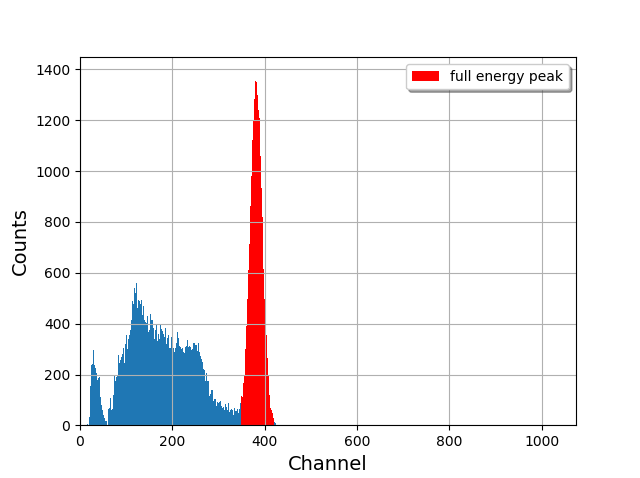
\includegraphics[width=.9\linewidth]{../Plots/attenuation_1.png}
  \caption{4 mm of copper}
\end{subfigure}%
 \vskip\baselineskip
\begin{subfigure}{.5\textwidth}
  \centering
  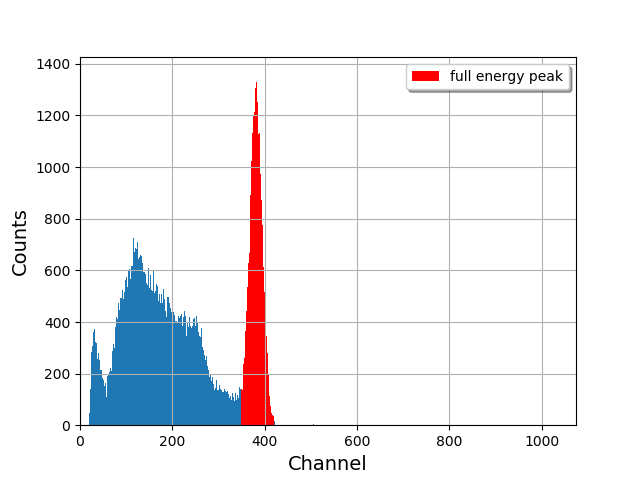
\includegraphics[width=.9\linewidth]{../Plots/attenuation_2.png}
  \caption{8 mm of copper}
\end{subfigure}%
\begin{subfigure}{.5\textwidth}
  \centering
  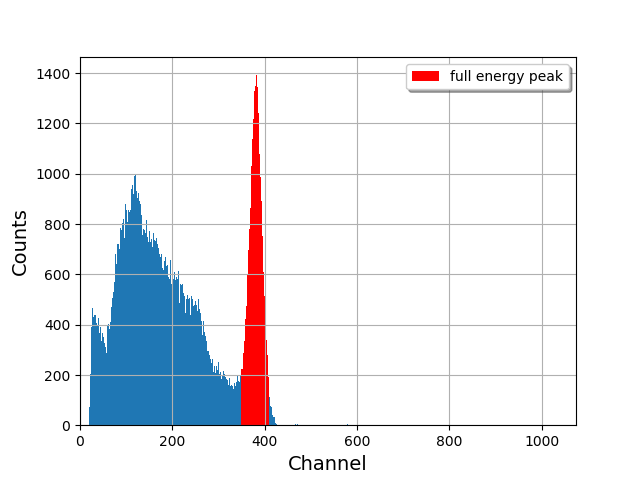
\includegraphics[width=.9\linewidth]{../Plots/attenuation_3.png}
  \caption{4 mm of copper}
\end{subfigure}%
 \vskip\baselineskip
\begin{subfigure}{.5\textwidth}
  \centering
  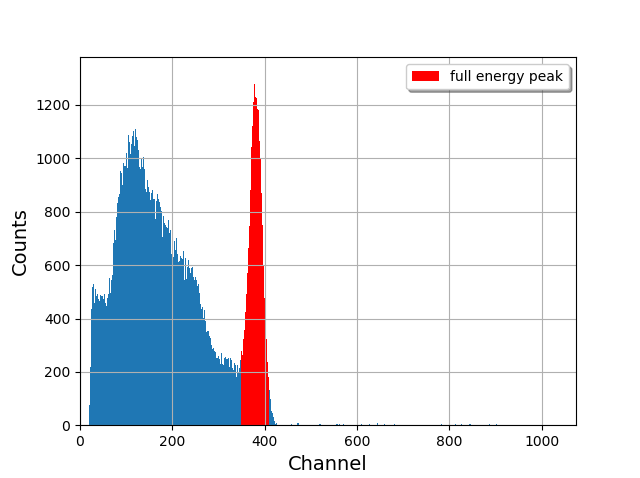
\includegraphics[width=.9\linewidth]{../Plots/attenuation_4.png}
  \caption{16 mm of copper}
\end{subfigure}%
\caption{Spectra of $^{137}$Cs with copper shielding}
\label{attenuation_spectra}
\end{figure}
Time for measurement was adjusted, that every peak has at least a maximum counting of 1000 events, to give us a better statistic.
Background radiation was again substracted from every spectrum.

We can see, that even the lowest shielding with 4 mm copper was enough to remove the beta-peak on the far left of the spectrum.
This can easily be explained with the low range of electrons in matter and was expected.
As attenuated quanitty, we used the full energy peak to calculate the counts per second from this peak.
This was calculated gain with Eq. \ref{gauss_area}.
The results can be seen in Table \ref{attenuation_values}.
\begin{table}[h]
\centering
\begin{tabular}{c |c }
\hline
Counts per second [s$^{-1}$] & thickness [mm] \\
\hline
334.1 & 0 \\
263.7 & 4 \\
208.6 & 8 \\
161.7 & 12 \\
127.1 & 16 \\
\hline
\end{tabular}
\caption{Attenuation through copper}
\label{attenuation_values}
\end{table}
Plotting this data enabled us to fit the values according to the function:
\begin{equation}
I(d) = I_0 e^{a \cdot d}
\end {equation}
With $a = \frac{\mu}{\rho}$.
Given the density of copper at $300$K ($8.96 \text{gcm}^{-3}$) made it possible to calculate the attenuation coefficient of copper from this fit-parameter.
The data and fit can be seen in Fig. \ref{attenuation_fit}
\begin{figure}[h]
  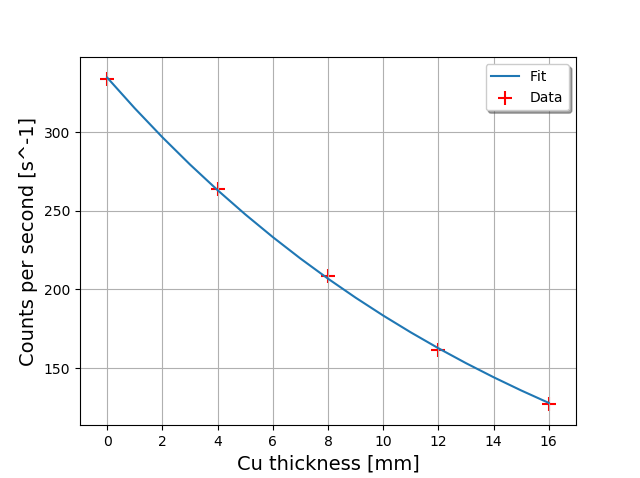
\includegraphics[width=\linewidth]{../Plots/attenuation.png}
  \caption{Data and fit of the attenuation}
  \label{attenuation_fit}
\end{figure}
We can directly see, that the data are well approximated through the exponential function.
The fit parameter $a$ was calculated to $a = (60.17 \pm 0.26)$.
We can now calculate the attenuation coefficient $(\mu = \frac{a}{\rho}$), which gives us:

$\mu = (6.715 \pm 0.029) \cdot 10^{-2}$ $\text{cm}^2 \text{g}^{-1}$

As a literature value for comparision, we got $\mu = 7.3 \cdot 10^{-2}\text{cm}^2 \text{g}^{-1}$ (Quelle xcom einfügen).
\clearpage

\section{Diskussion}

Alle Aufgabenteile konnten erfolgreich abgeschlossen werden.

Im Niedrigenergiebereich wurden fünf verschiedene Proben auf ihre Zusammensetzung untersucht.
Dabei konnten in der 153BeO die Teilchen $^{16}$O$^{1-}$, $^{9}$Be$^{16}$O$^{1-}$ und $^{12}$C$^{16}$O$^{1-}$ bzw. $^{28}$Si$^{1-}$ nachgewiesen werden.
In den anderen Proben konnten diverse andere Teilchen, darunter bereits erwähnte mit anderen Nukliden sowie AlO gefunden werden.
Zusätzlich wurden einige unbekannte Stoffe gefunden, die wir in diesem Praktikum nicht genauer identifizieren konnten.
Mit einer genauerem Untersuchung der Probe bzw. genaueren Wissen über potentiell vorkommende Elemente sollte das aber auch möglich sein.

Im Hochenergiebereich wurde nur eine Probe untersucht.
Bei dieser wurden die Nuklide $^{9}$Be, $^{10}$Be, $^{12}$C, $^{16}$O und $^{26}$Al in verschiedenen Ladungszuständen gefunden.
Hier ist teilweise eine recht große Ungenauigkeit zwischen berechneter Masse und dem Nuklid vorhanden.
Dies lässt sich zumindest teilweise auf die unbekannten Ungenauigkeiten der Messung zurückführen.
Möglicherweise wurden hier auch einzelne Ionen fehlgedeutet.
Mit Kenntnis der Ursache der Ungenauigkeiten könnte dies genauer werden.

Weiterhin wurde die Detektion und Identifikation von $^{10}\text{Be}$ in einer Gasgefüllten Ionisationsdetektor vorgenommen.
Eine Trennung von den meisten unerwünschten Nukliden die nach dem Beschleuniger auftreten erfolgt durch einen Ablenkmagneten und einen ESA.
Aber auch das Isotop $^{9}\text{Be}$ kann gefunden werden, obwohl man es eigentlich durch Vorselektion aussortieren wollte.
Als Ursache dafür wurde die Molekülbildung von $^{9}\text{Be}^{1}\text{H}^{2+}$ angeführt.
Die Identifikation ist trotz des Auftretens des Isobars $^{10}\text{B}$ möglich.
Es ist sogar möglich das Isobar quantitativ im Spektrum von $^{10}\text{Be}$ zu trennen, womit grundsätzlich eine genaue Bestimmung des Anteils des radioaktiven Isotops $^{10}\text{Be}$ möglich ist, und damit die eigentliche Altersbestimmung.

Die Anteilsbestimmung wurde im letzten Versuchsteil vorgenommen.
Die Konzentration des Radionuklides $^{10}$Be wurde dazu in vier verschiedenen Proben berechnet.
Die Ergebnisse dafür sind in Tab. \ref{dis_con} zu sehen.
\begin{table}[h]
\centering
\caption{Gemessene Werte zur Berechnung der $^{10}$Be Konzentration in den Proben.}
\begin{tabular}{|c |c| c|}
\hline
Probe& $\frac{\text{Atome}}{\si{\gram}}$ & mittlere Tiefe [cm] \\
\hline
KY13 &  $(\num{1.115} \pm \num{0.050}) \cdot 10^{6} $ & 47,5\\
KY14 &  $(\num{9.61} \pm \num{0.44}) \cdot 10^{5} $ & 57,5 \\
KY16 &  $(\num{7.66} \pm \num{0.36}) \cdot 10^{5} $ & 92,5\\
KY17 &  $(\num{6.23} \pm \num{0.33}) \cdot 10^{5} $ & 112,5\\
\hline
\end{tabular}
\label{dis_con}
\end{table}
Wir konnten feststellen, dass die Konzentration scheinbar linear mit zunehmender Tiefe abnimmt.
Dies haben wir so erklärt, dass $^{10}$Be durch Ereignisse mit kosmischer Strahlung entsteht und tieferliegende Proben aufgrund ihres Alters daher weniger $^{10}$Be enthalten müssen.
Nach dieser Erklärung sollte eigentlich ein exponentieller Abfall stattfinden, was wir aber weder ausschließen noch bestätigen können.
Weitere Proben zur Messung könnten diese Frage aber beantworten.
Eine Verfälschung der Proben durch hochenergetische Strahlung aus anderen Quellen ist potentiell möglich, würde aber nichts am Abnehmen der Konzentration ändern.
Eine Neutronenquelle im Inneren der Probe würde das Ergebnis entsprechend ändern können, ist aber unwahrscheinlich.


\nocite{*} % alle resourcen auflisten
\printbibliography

% ----- DOKUMENT ENDE -----

\end{document}
